\documentclass[letterpaper]{article} % DO NOT CHANGE THIS
\usepackage[submission]{aaai2027}  % DO NOT CHANGE THIS
% The serif, sans-serif, and monospaced fonts are loaded automatically by
% aaai2027.sty (newtxtext, helvet, courier). DO NOT add \usepackage{times},
% \usepackage{helvet}, \usepackage{courier}, or any other font package.
\usepackage[hyphens]{url}  % DO NOT CHANGE THIS
\usepackage{graphicx} % DO NOT CHANGE THIS
\urlstyle{rm} % DO NOT CHANGE THIS
\def\UrlFont{\rm}  % DO NOT CHANGE THIS
\usepackage{natbib}  % DO NOT CHANGE THIS AND DO NOT ADD ANY OPTIONS TO IT
\usepackage{caption} % DO NOT CHANGE THIS AND DO NOT ADD ANY OPTIONS TO IT
\frenchspacing  % DO NOT CHANGE THIS
%
% These are recommended to typeset algorithms but not required. See the subsubsection on algorithms. Remove them if you don't have algorithms in your paper.
\usepackage{algorithm}
\usepackage{algorithmic}

%
% These are recommended to typeset listings but not required. See the subsubsection on listing. Remove this block if you don't have listings in your paper.
\usepackage{newfloat}
\usepackage{listings}
\DeclareCaptionStyle{ruled}{labelfont=normalfont,labelsep=colon,strut=off} % DO NOT CHANGE THIS
\lstset{%
	basicstyle={\footnotesize\ttfamily},% footnotesize acceptable for monospace
	numbers=left,numberstyle=\footnotesize,xleftmargin=2em,% show line numbers, remove this entire line if you don't want the numbers.
	aboveskip=0pt,belowskip=0pt,%
	showstringspaces=false,tabsize=2,breaklines=true}
\floatstyle{ruled}
\newfloat{listing}{tb}{lst}{}
\floatname{listing}{Listing}

%
% Recommended for better-looking tables
\usepackage{booktabs}
\usepackage{multirow}

% Math and theorem environments
\usepackage{amsmath,amssymb,amsthm}
\newtheorem{proposition}{Proposition}
\newtheorem{lemma}{Lemma}

%
% Keep the \pdfinfo as shown here. There's no need
% for you to add the /Title and /Author tags.
\pdfinfo{
/TemplateVersion (2027.1)
}

% DISALLOWED PACKAGES
% \usepackage{authblk} -- This package is specifically forbidden
% \usepackage{balance} -- This package is specifically forbidden
% \usepackage{CJK} -- This package is specifically forbidden
% \usepackage{float} -- This package is specifically forbidden
% \usepackage{flushend} -- This package is specifically forbidden
% \usepackage{fullpage} -- This package is specifically forbidden
% \usepackage{geometry} -- This package is specifically forbidden
% \usepackage{hyperref} -- This package is specifically forbidden
% \usepackage{navigator} -- This package is specifically forbidden
% (or any other package that embeds links such as navigator or hyperref)
% \usepackage{indentfirst} -- This package is specifically forbidden
% \usepackage{layout} -- This package is specifically forbidden
% \usepackage{multicol} -- This package is specifically forbidden
% \usepackage{nameref} -- This package is specifically forbidden
% \usepackage{savetrees} -- This package is specifically forbidden
% \usepackage{setspace} -- This package is specifically forbidden
% \usepackage{stfloats} -- This package is specifically forbidden
% \usepackage{tabu} -- This package is specifically forbidden
% \usepackage{titlesec} -- This package is specifically forbidden
% \usepackage{tocbibind} -- This package is specifically forbidden
% \usepackage{ulem} -- This package is specifically forbidden
% \usepackage{wrapfig} -- This package is specifically forbidden
% DISALLOWED COMMANDS
% \nocopyright -- Your paper will not be published if you use this command
% \addtolength -- This command may not be used
% \balance -- This command may not be used
% \baselinestretch -- Your paper will not be published if you use this command
% \clearpage -- No page breaks of any kind may be used for the final version of your paper
% \columnsep -- This command may not be used
% \newpage -- No page breaks of any kind may be used for the final version of your paper
% \pagebreak -- No page breaks of any kind may be used for the final version of your paper
% \pagestyle -- This command may not be used
% \tiny -- This is not an acceptable font size.
% \vspace{- -- No negative value may be used in proximity of a caption, figure, table, section, subsection, subsubsection, or reference
% \vskip{- -- No negative value may be used to alter spacing above or below a caption, figure, table, section, subsection, subsubsection, or reference

\setcounter{secnumdepth}{0} %May be changed to 1 or 2 if section numbers are desired.

% The file aaai2027.sty is the style file for AAAI Press
% proceedings, working notes, and technical reports.
%

% Title

% Your title must be in mixed case, not sentence case.
% That means all verbs (including short verbs like be, is, using,and go),
% nouns, adverbs, adjectives should be capitalized, including both words in hyphenated terms, while
% articles, conjunctions, and prepositions are lower case unless they
% directly follow a colon or long dash
\title{PACT: Identity-Preserving Domain-Incremental Adaptation of Frozen Time-Series Foundation Models}
\author{
    %Authors
    % All authors must be in the same font size and format.
    Written by AAAI Press Staff\textsuperscript{\rm 1}\thanks{With help from the AAAI Publications Committee.}\\
    AAAI Style Contributions by Peter Patel Schneider,
    Sunil Issar,\\
    J. Scott Penberthy,
    George Ferguson,
    Hans Guesgen,
    Francisco Cruz\equalcontrib\corresponding,
    Marc Pujol-Gonzalez\equalcontrib\corresponding
}
\affiliations{
    %Afiliations
    \textsuperscript{\rm 1}Association for the Advancement of Artificial Intelligence\\
    % If you have multiple authors and multiple affiliations
    % use superscripts in text and roman font to identify them.
    % For example,

    % Sunil Issar\textsuperscript{\rm 2},
    % J. Scott Penberthy\textsuperscript{\rm 3},
    % George Ferguson\textsuperscript{\rm 4}\corresponding,
    % Hans Guesgen\textsuperscript{\rm 5}
    % Note that the comma should be placed after the superscript

    1101 Pennsylvania Ave, NW Suite 300\\
    Washington, DC 20004 USA\\
    % email address must be in roman text type, not monospace or sans serif
    proceedings-questions@aaai.org
%
% See more examples next
}

%Example, Single Author, ->> remove \iffalse,\fi and place them surrounding AAAI title to use it
\iffalse
\title{My Publication Title --- Single Author}
\author {
    Author Name
}
\affiliations{
    Affiliation\\
    Affiliation Line 2\\
    name@example.com
}
\fi

\iffalse
%Example, Multiple Authors, ->> remove \iffalse,\fi and place them surrounding AAAI title to use it
\title{My Publication Title --- Multiple Authors}
\author {
    % Authors
    First Author Name\textsuperscript{\rm 1,\rm 2}\equalcontrib,
    Second Author Name\textsuperscript{\rm 2}\equalcontrib,
    Third Author Name\textsuperscript{\rm 1}\corresponding
}
\affiliations {
    % Affiliations
    \textsuperscript{\rm 1}Affiliation 1\\
    \textsuperscript{\rm 2}Affiliation 2\\
    firstAuthor@affiliation1.com, secondAuthor@affilation2.com, thirdAuthor@affiliation1.com
}
\fi


\begin{document}

\maketitle

\begin{abstract}
Pretrained time-series foundation models (TSFMs) provide transferable
representations for classification, but deployed systems often face
operating conditions that arrive sequentially after training. Each new
condition may provide only a small labeled calibration set, and condition
identity may be unknown at inference. Fine-tuning shared parameters can
recover macro-$F_1$ on the new condition but can degrade previously observed
ones, while retention-focused methods often limit adaptation. We find that,
for frozen TSFM encoders, operating-condition shift is strongly
heterogeneous across local embedding regions: some regions move
substantially while others remain stable. This motivates correcting drift
locally rather than transforming the full representation. We introduce
\textbf{PACT} (\emph{\textbf{P}iecewise \textbf{A}daptation via
\textbf{C}hart \textbf{T}ransport}), a frozen-host adaptation method that
covers the source embedding space with local charts, learns lightweight
residual transports for each new condition, and routes inputs through the
accumulated transports while retaining an explicit identity path. The
encoder, classifier head, and previously learned transports remain frozen.
We further derive a margin-based condition under which a routed correction
preserves the original prediction. Across four sequential bearing-fault
operating conditions using only 5\% labeled calibration data and no
condition identity at test time, PACT maintains average macro-$F_1$ above
0.98. The same retention--adaptation pattern appears on human-activity
recognition and sleep-staging streams across multiple backbones.
\end{abstract}


\section{Introduction}
\label{sec:intro}

\begin{figure}[t!]
    \centering
    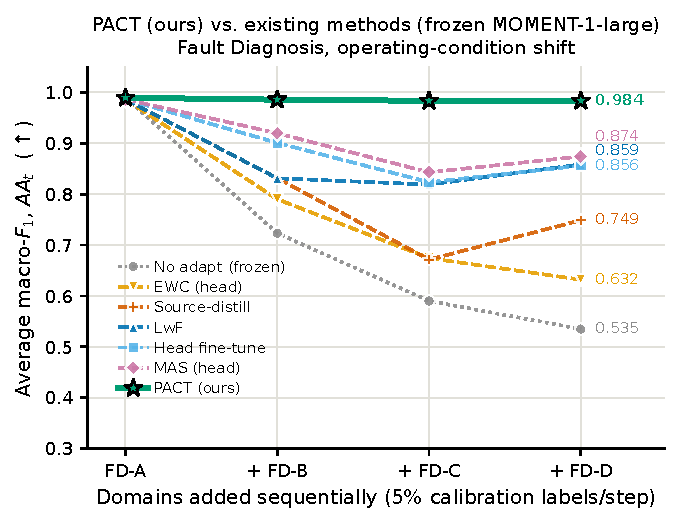
\includegraphics[width=.90\linewidth]{figures/fig_intro_chain_moment.pdf}
    \caption{PACT preserves average macro-$F_1$ during sequential adaptation
    on frozen MOMENT-large. Each new condition uses 5\% labels, and condition
    identity is unavailable at test time.}
    \label{fig:intro}
\end{figure}

Pretrained time-series foundation models (TSFMs)
\citep{goswami_moment_2024,moirai,ansari_chronos_2024,pmlr-v267-liu25be,shi_time-moe_2025}
provide general-purpose representations that transfer across temporal
domains and downstream tasks. A common deployment strategy is therefore
to freeze the pretrained encoder and train only a lightweight
classification head using task-specific labeled data. This approach is
data-efficient and preserves the reusable representation learned during
pretraining.

Real deployments, however, are rarely stationary. A fault-diagnosis
model may be trained under one combination of machine load, speed, and
operating environment, yet encounter different conditions throughout
the machine's service life. These conditions arrive sequentially, often
with only a small labeled calibration set, and their identity may be
unavailable at inference. The deployed classifier must consequently
recognize samples from every condition observed so far without being
told which condition generated each sample.

Frozen TSFM classifiers can fail sharply under such shifts. On a
bearing-fault benchmark, a classifier built on a frozen TSFM reaches
$0.997$ macro-$F_1$ on its source condition, while its macro-$F_1$ falls
to $0.43$ after an operating-condition change. Fine-tuning can recover
performance on the new condition, but it changes shared parameters and
can degrade earlier ones. Regularization-based continual-learning methods
constrain this degradation, but remain
subject to the stability--plasticity trade-off: weak constraints permit
adaptation but allow forgetting, whereas strong constraints retain the
source model but limit recovery on the new condition
\citep{ewc,mas,si,lwf}. Expandable methods reduce parameter interference
by allocating condition-specific modules, but commonly depend on hard
routing, explicit task cues, or reliable inferred condition identity
\citep{sprompts}. Such routing can be unreliable when conditions are mixed
and unlabeled at inference.

These limitations motivate a more restrictive deployment objective:
adapt to each newly observed condition without modifying the pretrained
encoder, the classifier head, or corrections learned for earlier
conditions. Freezing the host prevents adaptation from overwriting its
representation or decision geometry. It also isolates any remaining
degradation to the newly introduced correction and its routing
mechanism, rather than distributing it across shared model parameters.
Recent work has begun to study domain-incremental time-series classification
directly \citep{dualcd}; PACT addresses the complementary frozen-host regime,
where the pretrained encoder and head cannot be modified, only 5\% calibration
labels are available, and an exact identity path must be retained.

\paragraph{Operating-condition shift is locally concentrated.}
We investigate how the embedding space of a frozen TSFM changes across
operating conditions. The displacement is highly non-uniform: a subset
of representation regions moves substantially, while many regions
remain comparatively stable. A single global transformation can
therefore alter embeddings that require little or no correction. If
these embeddings already lie on the correct side of the frozen
classifier's decision boundary, unnecessary displacement can reduce
performance on previously well-classified conditions. Our measurements show
that a target-fitted global transform can reduce source margins and source
accuracy. This observation suggests that forgetting can arise not only from
learning new conditions, but also from applying adaptation at an
inappropriately coarse granularity.

\paragraph{Piecewise adaptation with a frozen host.}
Motivated by this observation, we introduce \textbf{PACT}
(\emph{\textbf{P}iecewise \textbf{A}daptation via \textbf{C}hart
\textbf{T}ransport}), a frozen-host method for sequential
operating-condition adaptation. PACT partitions the source embedding
space into local regions, termed \emph{charts}. For each newly observed
condition, it learns a lightweight residual transport for each chart
using only a small labeled calibration set. The transports are
identity-initialized and optimized through the frozen classifier head,
so adaptation moves shifted embeddings toward the decision geometry
already represented by the host rather than modifying that geometry.
Once learned, each transport is frozen; subsequent conditions add new
corrections without changing the encoder, head, or previous transports.

At inference, the condition identity is unknown. PACT therefore uses a
gate calibrated from in-distribution embeddings to softly route each
sample across the accumulated transports. An explicit identity path is
always retained, preserving access to the original frozen
representation. This design separates two sources of degradation.
Overwriting of the host and earlier transports is excluded because these
components never change. A prediction can differ from the original only
through the routing and transport applied to its embedding. In
particular, identity routing reproduces the original prediction exactly,
and we derive a margin condition under which even a non-identity routed
correction leaves the predicted class unchanged.

Routing is essential rather than auxiliary. Per-chart transports without
a gate can improve some shifts but harm others by applying unnecessary
corrections. In several configurations, ungated correction performs
below the unadapted source model. PACT therefore combines local correction
and identity-preserving routing as a single adaptation mechanism.

We evaluate PACT in a domain-incremental setting where operating
conditions arrive sequentially, only $5\%$ of each new condition is
labeled for calibration, and condition identity is unavailable at test
time. Across four operating conditions of a bearing-fault benchmark,
PACT maintains an average macro-$F_1$ of $0.984$ over all conditions seen
so far. It is the only evaluated method to remain above $98\%$ average
macro-$F_1$ as conditions accumulate, while baselines that update shared
parameters lose substantially on the retention--adaptation trade-off. We further
observe the same retention--adaptation pattern on human-activity
recognition and sleep-staging streams across multiple TSFM backbones.

Our contributions are as follows:

\begin{itemize}
    \item We formulate sequential operating-condition adaptation for
    frozen TSFM classifiers under few labeled calibration samples, no
    condition identity at inference, and the requirement to retain all
    previously observed conditions.

    \item We show that operating-condition shift is locally concentrated
    in the frozen embedding space and provide empirical evidence that
    global correction can damage regions requiring little adaptation.

    \item We introduce PACT, which combines identity-initialized
    per-chart transports with soft, identity-preserving routing while
    keeping the encoder, classifier head, and previous transports frozen.
    We also derive a margin-based condition under which the original
    prediction is preserved.

    \item We evaluate PACT across bearing-fault diagnosis,
    human-activity recognition, and sleep-staging streams with multiple
    TSFM backbones. PACT consistently improves new-condition performance
    while retaining earlier conditions, and our ablations show that
    routing is necessary for reliable piecewise adaptation.
\end{itemize}


\section{Related Work}
\label{sec:related}

\paragraph{Domain and test-time adaptation.}
Domain adaptation aligns source and target representations, while test-time
adaptation updates a deployed model from unlabeled target samples
\citep{dann,mmda,msda,tent,cotta,ecotta,eata}. Both optimize shared components
for the current distribution. PACT instead leaves the encoder and head
unchanged because test samples may come from any previously seen condition.

\paragraph{Continual and frozen-backbone learning.}
Regularization-based continual learning constrains parameter drift
\citep{ewc,mas,si,lwf}; rehearsal-free methods use prompts, prototypes, or
temporal distillation \citep{dualprompt,sprompts,dualcp,dt2w}. DualCD directly
studies domain-incremental time-series classification by updating a model
sequentially \citep{dualcd}, whereas PACT keeps the pretrained host and head
immutable. S-Prompts uses KNN to select one domain-specific input prompt per
sample and offers no exact original-prediction path. PACT instead soft-mixes
identity and condition transports, retains such a path, and corrects local
charts rather than the whole representation. Frozen-backbone methods such as
RanPAC, ADAM, and EASE construct classifiers or subspaces on fixed
representations, mostly for class-incremental learning
\citep{ranpac,adam,ease}. PACT addresses fixed-label operating-condition
streams with few labels, no condition identity, and no raw-series replay.

\paragraph{Source-free and few-label adaptation.}
SHOT and the time-series-specific MAPU adapt a source encoder using unlabeled
target data, with MAPU enforcing temporal consistency through imputation
\citep{shot,mapu}. They target a single source-to-target shift, violate (C4) by
modifying the encoder, and provide no retention mechanism over a stream. PACT
instead uses a small labeled calibration set while retaining the frozen host
and all earlier corrections.

\section{Method}
\label{sec:method}

\subsection{Setting}
\label{sec:setting}

We study domain-incremental continual learning for time-series classification
on top of a frozen pretrained encoder.

Let $x\in\mathbb{R}^{C\times L}$ denote a time series with $C$ channels and
length $L$. A pretrained encoder $f_\theta:\mathbb{R}^{C\times L}\to\mathbb{R}^{p}$
maps it to an embedding $z=f_\theta(x)$, and a head
$h_\phi:\mathbb{R}^{p}\to\mathbb{R}^{Y}$ maps that embedding to class logits over a
label set $\mathcal{Y}=\{1,\dots,Y\}$. The head is fit once on a source domain
$\mathcal{D}_0$ and is linear. Thereafter a stream of domains
$\mathcal{D}_1,\dots,\mathcal{D}_T$ arrives sequentially. All domains share the
label space and the underlying task. They differ only in input distribution,
induced by a change of operating condition, subject, or sensor.

Each domain is split into disjoint train/calibration and test subsets. When
domain $\mathcal{D}_d$ arrives we observe a small labeled \emph{calibration
set} $\mathcal{C}_d\subset\mathcal{D}^{\mathrm{train}}_d$ with
$|\mathcal{C}_d|=\rho\,|\mathcal{D}^{\mathrm{train}}_d|$ and $\rho=5\%$.
Earlier raw time series are never revisited, although source and calibration
embeddings are retained to refit the routing gate. Domain identity is available
during calibration and unavailable at test time; all reported scores use
held-out test splits.

We require a deployed model that, after the stream has advanced to domain $t$,
satisfies four constraints.
\textbf{(C1)} It classifies inputs drawn from any seen domain $j\le t$.
\textbf{(C2)} It receives no domain label at test time.
\textbf{(C3)} It should minimize degradation on earlier domains as the stream grows.
\textbf{(C4)} It never modifies $f_\theta$ or $h_\phi$, so the original
frozen-host mapping remains exactly available through the identity path.

Constraint (C4) is what separates this setting from fine-tuning. A large
pretrained model retrained on a $5\%$ calibration slice can overfit that slice
and distort the representation that made it valuable. Our design takes the
encoder and the head as immutable and asks what can be done in the
$p$-dimensional embedding space alone.

\paragraph{Time-series foundation models as the frozen backbone.}
Our primary instantiation takes $f_\theta$ to be a pretrained time-series
foundation model (TSFM) and fits $h_\phi$ by linear probing on $\mathcal{D}_0$,
with no end-to-end training at any stage. Two adjustments make a
forecasting-pretrained encoder usable as a classifier.

First, \emph{multi-window pooling}. A TSFM has a fixed context length $P$. A
series with $L>P$ is split into $W$ windows $\{x^{(w)}\}$ of length $P$ and the
window embeddings are mean-pooled,
\begin{equation}
z \;=\; \frac{1}{W}\sum_{w=1}^{W}f_\theta\big(x^{(w)}\big).
\label{eq:pooling}
\end{equation}
This processes the full sequence without downsampling within each window. The
common alternative, downsampling the series to length $P$, may suppress
high-frequency patterns that are informative for distinguishing operating
conditions.

Second, \emph{embedding standardization}. Raw transformer embeddings have
strongly anisotropic per-coordinate scales. We standardize with source-fit
statistics $(m,s)$,
\begin{equation}
z \;\leftarrow\; (z-m)\oslash s ,
\label{eq:standardize}
\end{equation}
where $\oslash$ is elementwise division. This makes Euclidean geometry in
$\mathbb{R}^{p}$ less sensitive to coordinate scale, which every subsequent
component depends on.
Multivariate inputs are embedded channel-independently and averaged.

Nothing that follows uses any property of $f_\theta$ beyond
Eqs.~\eqref{eq:pooling}--\eqref{eq:standardize}. The method applies unchanged to
a task-specialist backbone trained end-to-end on $\mathcal{D}_0$.

\paragraph{Notation.}
We write $Z_0=\{f_\theta(x)\}_{x\in\mathcal{D}_0^{\mathrm{train}}}$ for the source embeddings and
$Z_d$ for the calibration embeddings of domain $d$. We write $A_{t,j}$ for the
macro-$F_1$ score on the held-out test split of domain $j$ after the model has
been adapted through domain $t$, for $j\le t$.

%---------------------------------------------------------------------
\subsection{Distribution Shift Acts Locally}
\label{sec:locality}

The design of \textsc{PACT} follows from a single empirical observation, which
we state and then measure. \emph{A change of operating condition does not
displace the representation manifold uniformly. It leaves some regions almost
fixed and transports others substantially.}

If this holds, a single global affine correction may be insufficient when
different regions shift by different amounts. Such a map can also move source
embeddings that did not need correction, and that collateral change can
contribute to degradation on earlier domains.

We make the claim falsifiable with three measurements, reported in
Fig.~\ref{fig:locality}. All three are computed on source embeddings partitioned
into $K$ regions by $k$-means, with centroids $\{\mu_c\}_{c=1}^{K}$ and hard
assignment $\kappa(z)=\arg\min_c\lVert z-\mu_c\rVert_2$.

\paragraph{(a) Damage is heterogeneous across charts.}
For chart $c$ and target domain $d$, let $A_c(\mathcal{D})$ be the macro-$F_1$
of the frozen pair $(f_\theta,h_\phi)$ restricted to samples of $\mathcal{D}$
assigned to chart $c$. The chart-conditional degradation is
\begin{equation}
\delta_c^{(d)} \;=\; A_c(\mathcal{D}_0)\;-\;A_c(\mathcal{D}_d).
\end{equation}
Were shift global, $\{\delta_c^{(d)}\}_c$ would be near-constant in $c$. It is
not. Its coefficient of variation across supported charts is large, and a
nontrivial fraction of supported charts satisfy $\delta_c^{(d)}\approx 0$.

\paragraph{(b) One affine map cannot fit the shift, several can.}
Fit the best single affine correction on the calibration set by minimizing the
frozen-head risk,
\begin{equation}
\mathcal{R}_{\mathrm{glob}}(d)
=
\min_{W,b}\;
\frac{1}{|\mathcal{C}_d|}\!\!\sum_{(x,y)\in\mathcal{C}_d}\!\!
\ell_{\mathrm{CE}}\big(h_\phi(Wz+b),\,y\big),
\end{equation}
and compare it against a piecewise-affine correction with one map per chart.
For chart $c$, write
$\ell_c(z,y)=\ell_{\mathrm{CE}}(h_\phi(W_cz+b_c),y)$. Then
\begin{equation}
\mathcal{R}_{\mathrm{atlas}}(d;K)
=
\min_{\{W_c,b_c\}}\;
\frac{1}{|\mathcal{C}_d|}\!\!\sum_{(x,y)\in\mathcal{C}_d}\!\!
\ell_{\kappa(z)}(z,y).
\end{equation}
All $K$ values use the same 5\% stratified calibration split for fitting and the
same disjoint domain test split for evaluation. Each affine map has $p^2+p$
parameters and is regularized toward the identity with weight $10^{-3}$; the
$K$-map model therefore has $K(p^2+p)$ parameters. Figure~\ref{fig:locality}(b)
reports the held-out residual $1-F_1$, not training loss. The residual drops
sharply once local maps are introduced and is nearly saturated by
$K\!\approx\!16$, supporting a piecewise model of the observed shift.

\paragraph{(c) A target-fitted global map can degrade source margins.}
Let $\Psi_d^{\mathrm{glob}}(z)=W^{\star}z+b^{\star}$ be the fitted global map and
let $m(z)$ denote the frozen head's true-class margin. We measure the mean
chart-wise margin change
\begin{equation}
\Delta m_c(\mathcal D;d)
=
\mathop{\mathbb{E}}_{z\in Z(\mathcal D),\;\kappa(z)=c}
\left[m\!\left(\Psi_d^{\mathrm{glob}}(z)\right)-m(z)\right].
\end{equation}
The map fitted to the most shifted target improves several target charts, but
reduces the source margin in most source charts and lowers source macro-$F_1$
from $0.998$ to $0.426$. This illustrates one mechanism associated with source
degradation: a global correction can alter already-correct embeddings.

\paragraph{Consequences.}
Three design commitments follow directly, and we adopt no others.
\textbf{(i)} Corrections must be \emph{local}, defined on charts rather than on
the whole space. \textbf{(ii)} Each correction must be \emph{anchored at the
identity}, so that a chart needing no change receives none. \textbf{(iii)} A
correction learned for one domain must be \emph{frozen}, so that later domains
cannot reach back and displace it.

\begin{figure*}[t]
\centering
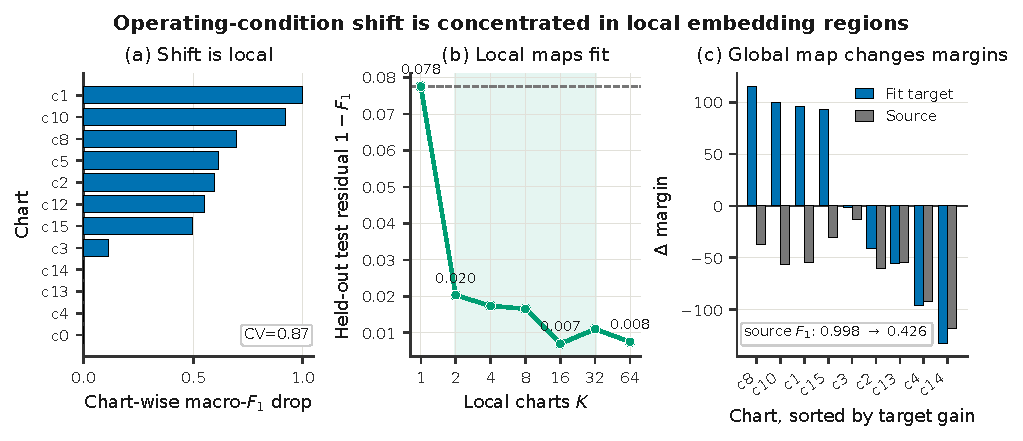
\includegraphics[width=.92\textwidth]{figures/fig_locality.pdf}
\caption{\textbf{Distribution shift acts locally.}
(a)~Per-chart macro-$F_1$ drop is highly heterogeneous among supported charts;
``n/a'' marks charts with no target-domain support.
(b)~Maps are fitted on the labeled calibration split and evaluated on the
disjoint test split; the residual falls sharply as local capacity is introduced,
supporting a piecewise model of the observed shift.
(c)~A global map fitted to the most shifted target changes target and source
margins differently and reduces source macro-$F_1$, illustrating one mechanism
associated with source degradation; charts without target support are omitted.}
\label{fig:locality}
\end{figure*}

%---------------------------------------------------------------------
\subsection{An Atlas of Frozen Transports}
\label{sec:atlas}

The frozen head $h_\phi$ partitions $\mathbb{R}^{p}$ into fixed decision regions.
The encoder places many source embeddings inside the correct ones. A shifted
domain can place them elsewhere. Adaptation, under (C4), therefore cannot mean moving the
decision regions. It can only mean \emph{transporting shifted embeddings back
into a geometry that never moves}. This is the operation \textsc{PACT} learns,
and it learns it one region at a time.

\paragraph{Charts.}
We compute $\{\mu_c\}_{c=1}^{K}$ once on $Z_0$ by $k$-means and never update
them. We call these local Voronoi regions \emph{charts}. Each chart is
represented by a centroid, and an embedding is assigned to its nearest chart,
\begin{equation}
\kappa(z)=\arg\min_{c\in\{1,\ldots,K\}}\lVert z-\mu_c\rVert_2.
\label{eq:chart-assignment}
\end{equation}
The same source-fit assignment is used for calibration and inference. Domain
routing remains soft even though chart selection is discrete.

\paragraph{Transports.}
For each domain $d\ge 1$ and chart $c$, we learn an affine map
\begin{equation}
T_c^d(z)=W_c^d z+b_c^d,
\qquad
\Delta_c^d(z)=T_c^d(z)-z .
\label{eq:transport}
\end{equation}
We initialize $W_c^d=I$ and $b_c^d=0$, so the residual is initially zero and
$T_c^d(z)=z$. The source branch is the fixed identity
$T_c^0(z)=z$. We also evaluate the low-rank residual
$T_c^d(z)=z+B_c^dA_c^dz$, with rank $r=8$ \citep{lora}.

\paragraph{Training a transport bank.}
Domain identity is known during calibration, so transports are fit without any
routing. We minimize the frozen-head risk with an identity anchor,
\begin{align}
\mathcal{L}_{\mathrm{tr}}\big(T^{d}\big)
&=
\frac{1}{|\mathcal{C}_d|}\!\!\sum_{(x,y)\in\mathcal{C}_d}\!\!
\ell_{\mathrm{CE}}\Big(h_\phi\big(T_{\kappa(z)}^{d}(z)\big),\,y\Big)
\notag\\
&\quad+\;
\lambda\sum_{c=1}^{K}
\left(\lVert W_c^d-I\rVert_F^2+\lVert b_c^d\rVert_2^2\right).
\label{eq:transport-loss}
\end{align}
Here $z=f_\theta(x)$ and $\lambda=10^{-3}$. This parameter-space identity
anchor discourages large residual corrections but does not impose a pointwise
output bound. For the low-rank variant, the corresponding penalty is
$\lambda\sum_c\lVert B_c^d\rVert_F^2$.

Gradients reach only $\Delta^{d}$. The encoder, the head, and every transport
bank $\{\Delta^{j}\}_{j<d}$ receive no updates at any point. Once
$\mathcal{L}_{\mathrm{tr}}$ has converged, $\Delta^{d}$ is frozen and appended to
the atlas. The model therefore \emph{accumulates} domains. It does not overwrite
them.

%---------------------------------------------------------------------
\subsection{Routing Without Domain Identity}
\label{sec:routing}

At test time the domain is unknown, so the model must decide which transports to
apply from the embedding alone. For each chart $c$, a two-layer MLP
$g_c:\mathbb{R}^p\rightarrow\mathbb{R}^{T+1}$ predicts a logit for the source
identity branch and every adapted domain. The hidden layer has width 64, ReLU,
and dropout 0.2. The gate is trained to classify domain identity using source
embeddings and the retained calibration embeddings of all seen domains; domain
classes are balanced by oversampling. When a domain arrives, the gate output is
expanded and the gates are refit on this accumulated embedding buffer.

\paragraph{Soft domain routing.}
For $c=\kappa(z)$, the routing distribution at temperature $\tau=0.5$ is
\begin{align}
\pi_{c,d}(z)
&=
\operatorname{softmax}_{d}\!\left(g_c(z)/\tau\right).
\label{eq:gate}
\end{align}
The source index $d=0$ is always present, so the original frozen-host mapping is
an explicit branch in every mixture.

\paragraph{Prediction.}
Combining Eqs.~\eqref{eq:chart-assignment}--\eqref{eq:gate}, and using
$\Delta^{0}_{c}\equiv 0$ to drop the source residual,
\begin{align}
\hat z
&=
z
+ \sum_{d=1}^{T} \pi_{\kappa(z),d}(z)\,
\Delta^{d}_{\kappa(z)}(z), \notag\\
\hat y
&= \arg\max_{y}\,\big[h_\phi(\hat z)\big]_y .
\label{eq:inference}
\end{align}
Domain routing is soft: an ambiguous sample blends transport outputs rather than
committing to one domain branch. The chart index is selected by nearest-centroid
assignment.

\paragraph{Cost.}
The encoder is evaluated once. Chart assignment costs $\mathcal{O}(Kp)$, gate
evaluation costs $\mathcal{O}(p+T)$ for the selected chart, and the mixture
evaluates one affine transport per adapted domain.

\paragraph{Sequential update.}
Absorbing a new domain computes embeddings for its 5\% calibration slice, fits
and freezes the fresh transport bank $T^d$, and refits only the routing gates on
the source and accumulated calibration embeddings. The encoder, head, and all
earlier transports remain unchanged; raw time series are not retained.

%---------------------------------------------------------------------
\subsection{Conditions for Prediction Preservation}
\label{sec:guarantee}

Freezing the encoder, the head, and all past transports removes every channel by
which a new domain could damage an old one, with a single exception. The gate may
route an old-domain embedding to a new domain's transport. We now show that even
this residual channel is bounded, and that the bound is controlled by two
quantities the model already regulates.

Let $h_\phi$ be $L$-Lipschitz coordinatewise with respect to $\lVert\cdot\rVert_2$,
which for a linear head gives $L=\max_y \lVert \phi_y\rVert_2$. Define the margin
of an embedding $z$ with true label $y^{\star}$,
\begin{equation}
m(z)
=
\big[h_\phi(z)\big]_{y^{\star}}
-
\max_{y\neq y^{\star}}\big[h_\phi(z)\big]_{y},
\end{equation}
and define the identity mass assigned to $z$ as
\begin{equation}
\pi_0(z) \;=\; \pi_{\kappa(z),0}(z) \;\in\; [0,1].
\end{equation}
Finally, define the largest available residual correction at $z$ as
\begin{equation}
B(z) \;=\; \max_{d\in\{1,\ldots,T\}}
\big\lVert\Delta^d_{\kappa(z)}(z)\big\rVert_2.
\end{equation}
Unlike the parameter-space identity penalty, $B(z)$ is a pointwise quantity
that can be computed directly for any embedding and fitted atlas.

\begin{proposition}[Margin-bounded non-degradation]
\label{prop:margin}
Let $z$ be any embedding that the frozen model classifies correctly, so
$m(z)>0$. Then
\begin{equation}
\big\lVert \hat z - z \big\rVert_2 \;\le\; \big(1-\pi_0(z)\big)\,B(z) ,
\end{equation}
and \textsc{PACT} classifies $z$ correctly whenever
\begin{equation}
\big(1-\pi_0(z)\big)\,B(z) \;<\; \frac{m(z)}{2L}.
\label{eq:margin-condition}
\end{equation}
In particular, if $\pi_0(z)=1$ then $\hat z = z$ exactly and the prediction is
identical to that of the original frozen model.
\end{proposition}

The proof is given in the supplementary material. The displacement bound is
unconditional by definition of $B(z)$; prediction preservation remains
conditional on Eq.~\eqref{eq:margin-condition}. This is not a claim of zero
forgetting: degradation requires both low identity mass and a sufficiently
large residual correction. The identity anchor in
Eq.~\eqref{eq:transport-loss} discourages the latter, while both factors in the
condition are measurable after fitting.

\paragraph{The gap that measures routing error.}
Because misrouting is the sole degradation channel left by the frozen host, it
can be isolated. Let
$A^{\mathrm{orc}}_{T,j}$ be the score obtained when the true domain label is used
in place of Eq.~\eqref{eq:gate}, and $A_{T,j}$ the score under the deployed gate.
The \emph{oracle-routing gap}
\begin{equation}
\mathrm{ORG}_{j} \;=\; A^{\mathrm{orc}}_{T,j} - A_{T,j}
\end{equation}
is a diagnostic of the part of PACT's residual error attributable to routing
rather than to the learned transports themselves.

%---------------------------------------------------------------------
\subsection{Memory and Parameter Cost}
\label{sec:cost}

\textsc{PACT} stores $Kp(p{+}1)$ affine parameters per domain; the rank-$r$
variant uses $2Krp$. A chart gate with hidden width $q$ has
$(p{+}1)q+(q{+}1)(T{+}1)$ parameters and is instantiated independently for each
chart. Gate refitting retains source-train and calibration embeddings, requiring
$p(|Z_0|+\sum_d|Z_d|)$ floats; no raw time series are retained.

\section{Experiments}
\label{sec:experiments}

\begin{figure*}[t]
\centering
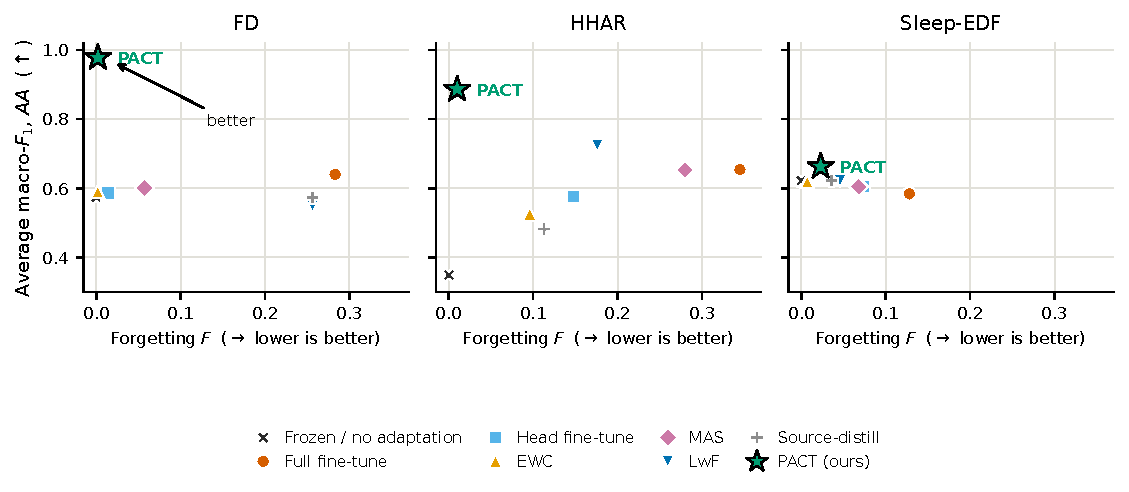
\includegraphics[width=.92\textwidth]{figures/fig_tradeoff.pdf}
\caption{\textbf{Macro-$F_1$--forgetting trade-off on the domain-incremental
chain (TSLANet backbone).} Top-left is best. PACT ($\star$) combines high
average macro-$F_1$ with low measured forgetting on all three streams. The
frozen baseline has zero forgetting by construction but weak adaptation.
ORTCL results are reported in Supplementary Table~2.}
\label{fig:tradeoff}
\end{figure*}

\subsection{Setup}
\label{sec:setup}

\paragraph{Benchmarks.}
We evaluate on three time-series classification benchmarks spanning
distinct shift types: \textbf{FD} (Paderborn bearing fault diagnosis; 4 operating
conditions, 3 classes, length 5120), \textbf{HHAR} (human activity recognition;
9 device/subject domains, 6 classes, length 128), and \textbf{Sleep-EDF}
(sleep-stage classification; 17 subject domains, 5 classes, length 3000)
\citep{paderborn,stisen_hhar_2015,kemp_sleep_2000}.

\paragraph{Protocols.}
We use two protocols. The \emph{pairwise} protocol follows
AdaTime \citep{adatime}: a model is adapted from a single source to a single target
operating condition, averaged over 10 source$\rightarrow$target shifts per
dataset; this is the native setting of UDA/TTA baselines. The
\emph{domain-incremental chain} protocol---the setting PACT
targets---presents all domains of a dataset sequentially, so that
forgetting on earlier domains is measured directly after the full stream.
Pairwise runs refit the source model for each ordered source--target pair and
then average across pairs; chain runs fit one fixed source model and follow one
complete domain order. Their frozen/source-only scores are therefore not
expected to match (for example, HHAR averages many pairwise sources but the
chain begins from User~0).

\paragraph{Backbones.}
We instantiate PACT on two specialist encoders (TSLANet, PatchTST)
\citep{eldele_tslanet_2024,nie_time_2022} and
five \emph{frozen} time-series foundation models (MOMENT-1-large,
Chronos-Bolt, Sundial, Time-MoE, Moirai)
\citep{goswami_moment_2024,ansari_chronos_2024,pmlr-v267-liu25be,shi_time-moe_2025,moirai}.

\paragraph{Baselines.}
Baselines fall into four families: unsupervised
domain adaptation (DANN, Deep~CORAL, MMDA, and the semi-supervised
DANN\textsuperscript{\dag}/CDAN\textsuperscript{\dag})
\citep{dann,deepcoral,mmda,cdan},
test-time adaptation (TENT), fine-tuning references (full and head-only),
and continual learning (EWC, MAS, LwF, source-distillation, ORTCL)
\citep{tent,ewc,mas,lwf,ortcl}. The dagger variants, fine-tuning methods,
continual-learning baselines, and PACT receive the same stratified 5\% labeled
target split. Unsupervised DA and TTA use target training inputs without labels.
Source-distillation is our constructed baseline: target cross-entropy is
combined with KL distillation from the frozen source model.

\paragraph{Metrics.}
Let $A_{t,j}$ be the macro-$F_1$ on domain $j$ after adapting through domain $t$. After the full stream ($t=T$) we report
\emph{Average macro-$F_1$}
$\mathrm{AA}=\frac{1}{T+1}\sum_{j=0}^{T}A_{T,j}$\;($\uparrow$);
\emph{Backward Transfer}
$\mathrm{BWT}=\frac{1}{T}\sum_{j=0}^{T-1}(A_{T,j}-A_{j,j})$
($\uparrow$; negative values indicate net degradation);
\emph{Forgetting relative to peak performance}
$F=\frac{1}{T}\sum_{j=0}^{T-1}
\max(0,\max_{j\le l<T}A_{l,j}-A_{T,j})$\;($\downarrow$, 0 = none);
and \emph{Relative Forgetting}
$\mathrm{RF}=\frac{1}{T}\sum_{j=0}^{T-1}
\frac{\max(0,\max_{j\le l<T}A_{l,j}-A_{T,j})}
{\max_{j\le l<T}A_{l,j}+\epsilon}$.
We use $\epsilon=10^{-9}$ in RF.
Chain results are single runs with seed 42; they are not averages over seeds.
Full per-method numbers for every figure below are provided in the
supplementary material.

%---------------------------------------------------------------------
\subsection{PACT Retains the Source and Recovers the Drift}
\label{sec:main-results}
Figure~\ref{fig:tradeoff} places every method on the macro-$F_1$--forgetting
plane for the domain-incremental chain (TSLANet backbone). The desirable
region is the top-left: high average macro-$F_1$ with near-zero forgetting.
PACT is the only evaluated adapting method that occupies it on all three benchmarks.
Host-modifying baselines are pushed down-and-right along a visible
trade-off: full fine-tuning and LwF recover some new-condition performance but forget
heavily ($F\!\ge\!0.25$ on FD), whereas the least-forgetting baselines
(EWC, head-tuning) limit forgetting largely by staying close to the
non-adapted model and never recover the drift.

On FD, PACT reaches AA $= 0.978$ with $F = 0.002$, while the
next-best baseline (MAS) achieves only $0.601$. On HHAR with 9 domains,
PACT attains $0.886$ with $F=0.010$ while all baselines remain below $0.723$.
On Sleep-EDF, PACT leads at $0.663$ with $F=0.023$ against a best baseline of
$0.622$.
On the pairwise AdaTime benchmark, PACT attains the best AA on FD ($0.981$)
and HHAR ($0.963$) while holding $F\!\le\!0.001$. On Sleep-EDF, PACT reaches
$0.715$, behind source-distillation at $0.721$, under the same 5\%
target-label budget.

We note one honest exception: on HHAR with frozen MOMENT, LwF restricted to the head reaches
marginally higher average macro-$F_1$ than PACT ($0.646$ vs.\ $0.627$) but at roughly
$3\times$ the forgetting ($F$: $0.051$ vs.\ $0.018$)---the one setting in the
paper where a baseline is not strictly dominated on both axes.

%---------------------------------------------------------------------
\subsection{PACT Is Backbone-Agnostic, Including Frozen TSFMs}
\label{sec:backbones}
Because PACT only requires an embedding and a frozen head, it applies
unchanged to specialist encoders and to forecasting-pretrained TSFMs used
purely as frozen feature extractors. Across seven backbones,
measured forgetting remains low
($F\!\le\!0.025$ everywhere). The two backbone families are complementary:
the frozen TSFMs (MOMENT, Chronos-Bolt, Sundial, Moirai) cluster at the top
on FD (up to $0.984$), while the lighter specialist TSLANet is strongest on
HHAR ($0.886$) and Sleep-EDF ($0.663$); Time-MoE trails the other TSFMs on FD ($0.943$) but is
still comfortably above the specialist PatchTST. This indicates that PACT's
retention behavior transfers across different embedding backbones, and
that a TSFM that remains fully frozen during adaptation becomes a
competitive continual classifier under PACT.
The full backbone plot and table are in the supplementary material.

%---------------------------------------------------------------------
\subsection{Ablation: The Gate Is a Necessity, Not a Refinement}
\label{sec:ablation}
The FD component ablation isolates each component.
Macro-$F_1$ rises monotonically from the frozen head ($0.574$/$0.535$ for
TSLANet/MOMENT), to full fine-tuning ($0.640$), to
ungated adapters ($0.748$/$0.879$), to full PACT ($0.978$/$0.984$).
Among the adapter variants, only gated PACT combines this recovery with
$F\!\le\!0.002$; ungated adapters reach $F=0.032/0.113$ and full fine-tuning
reaches $F=0.283$. Adapters supply plasticity; the gate converts that
plasticity into lower-forgetting accumulation.

Gate ablations explain why. Soft-mixture routing matches or beats hard $\arg\max$
routing and sits just below the oracle (perfect-routing) ceiling. Because the
host and past transports are frozen, the soft--oracle gap diagnoses the error
attributable to domain routing; that gap is
0.004/0.033/0.001 on FD/HHAR/Sleep-EDF with TSLANet, and the larger HHAR
gap is precisely where routing is hardest---localizing the residual forgetting
to a single, interpretable cause rather than to backbone drift.
The full ablation figure and tables are in the supplementary material.

%---------------------------------------------------------------------
\subsection{Robustness and Label Efficiency}
\label{sec:robustness}
PACT is stable over the tested hyperparameter ranges on the FD chain:
average macro-$F_1$ stays in $0.968$--$0.978$ for
$K\in\{4,\dots,64\}$ and in $0.971$--$0.979$ for
$\tau\in[0.1,2.0]$; full-affine and rank-8 residual transports differ by
$0.007$ AA.
With frozen MOMENT, average macro-$F_1$ generally increases with the calibration budget
(FD rises from $0.954$ at 1\% to $0.993$ at 20\%), and forgetting remains
below $0.025$ throughout the sweeps. Full curves and order-sensitivity
tables are in the supplementary material.

%---------------------------------------------------------------------
\section{Conclusion}
\label{sec:conclusion}

We introduced PACT, a frozen-host method for sequential operating-condition
adaptation of time-series classifiers. The key observation is that
distribution shift is locally concentrated in the embedding space: some
regions move substantially while others remain stable. PACT exploits this
by learning lightweight, identity-initialized transports on local charts
and softly routing test samples through the accumulated atlas, with the
source identity path always retained. The encoder, classifier head, and
all previously learned transports remain frozen, so changes on earlier domains
can arise only from the refitted gate and its mixture weights.

Across bearing-fault diagnosis, human-activity recognition, and sleep-staging
streams with seven backbones spanning task-specialist encoders and frozen
time-series foundation models, PACT achieves the strongest average
retention--adaptation trade-off in most settings, while retaining consistently
low forgetting. On the FD benchmark with frozen MOMENT, it maintains $0.984$
average macro-$F_1$ after four sequential conditions with just 5\% calibration
labels per step and no condition identity at test time. The HHAR/MOMENT case,
where LwF attains slightly higher macro-$F_1$ with higher forgetting, marks the
main exception rather than being hidden by the aggregate trend.

The method has clear limits. When the number of domains is very large and
calibration per domain is extremely sparse, the learned gate may not
separate overlapping distributions; the HHAR results ($0.886$ with TSLANet
but $0.627$ with frozen MOMENT) show that gate quality depends on the
separability of the underlying embeddings.
Hard nearest-centroid assignment can misroute embeddings across chart
boundaries; soft top-$k$ assignment, multi-layer chart discovery, and
session-level routing remain important extensions.

\bibliography{aaai2027}

\end{document}
